%==========================================================================================================================
% (c) Vojtěch Kulička, 2010

\chapter{Introduction}
Human is a social creature and likes to chat, share feelings and ideas. At first we managed to do so by making simple sounds. Those sounds later on developed into words. Then much later the human race started to feel the need to record what we were thinking. We made up symbols and started to write. As the society grew and spread, we wanted to communicate with people from other tribes and villages. At first we would travel and use spoken words, but as the distances grew we figured we can have our thoughts delivered in writing. Mail was born. In 1844 telegraph was invented by Samuel Morse followed by telepthone in 1874 by Alexander Graham Bell. And finally in 1969 the Internet was created. All of these inventions aimed to provide means of communication to satisfy the needs of the evolving society.  

In the early days of the Internet email was the main means of communication. And just like regular mail people would have their electronic mailboxes to which the emails were delivered. Email was a huge step forward for it provided a way to almost instantly deliver text from one place to another regardless of the distance for free. The main disadvantage of email is that people had to check their mailboxes read new mail and then reply. It is just neither fast nor convenient enough for team cooperation when team members are far apart. For those and other purposes like chatting Instant Messenger programs were introduced.    

An IM program offers realtime communication between two people via text messages that are delivered from one user to another instantly. Instant messangers became very popular and started adding on features like multiuser chat, various games and most importantly VoIP(Voice over IP) support. VoIP capable IM like skype have become extremely popular at first for making it possible for people to call each other for free over the internet. Later video conferencing capability was added, so you could talk and see you colleague at the same time. One more thing comes in extremely handy when working in a team - a whiteboard.

At this time there is no usable IM providing VoIP and shared whiteboard for GNU/Linux. This thesis aims to add VoIP support to an existing XMPP client with shared board called Makneto. Makneto was created by Jaroslav Řezník as a master's thesis in 2008. At this point it is using iris library for XMPP communication. The shared board data is also transferred over XMPP. One of the goals of this thesis is to port Makneto to telepathy, which is now a very reliable and robust library for communication for numerous protocols.  

The following chapter gives a detailed description of the current version of program Makneto. We will find out about it's architecture, strengths and weaknesses. 

Chapter number three focuses on XMPP/Jabber communication protocol. It talks about it's features and limitations. 

Chapter four is about Telepathy communiation framework, how it works, what it consists of. There is also a description of a IM client application Empathy based on Telepathy. 

Current audio and video streaming protocols are listed and discussed in chapter five. Based on this chapter a suitable protocol is chosen for the implementation.

Finally the implementantion of VoIP into Makneto is in chapter six.  


\chapter{Makneto}

% =========================================================================================================================
% =========================================================================================================================

\chapter{XMPP}

% =========================================================================================================================
% =========================================================================================================================

\chapter{Telepathy}
Telepathy is a modular communications framework for building real-time communication applications. It supports numerous communication protocols as plugable backends e.g XMPP/Jabber(telepathy-gabble), SIP(telepathy-sofiasip), MSN(telepathy-butterfly) etc. Each of telepathy's components runs in a separate process as desktop service and communicates via D-Bus. The components are shared by telepathy clients. For example if there are two clients using XMPP they both use the same instance of telepathy-gabble. To get a better idea of how this concept works take a look at figure ~\ref{fig:telepathyArchitecture}.\cite{TPWiki} 

\begin{figure}[ht]
\begin{center}
	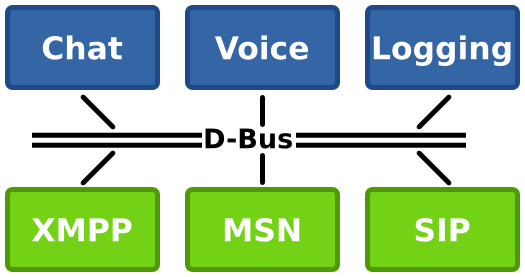
\includegraphics[width=10cm]{fig/telepathy-architecture-overview.png}
	\caption{Telepathy architecture\cite{TPWiki}}
	\label{fig:telepathyArchitecture}
\end{center}
\end{figure}


There are several features making telepathy very useful as a communications framework.

\begin{itemize}

	\item {\bf Robustness} - all the components are independent. If one crashes, others will not be affected

	\item {\bf Ease of development} - the components can be replaced without having to stop the service 

	\item {\bf Language independence} - since telepathy components use D-Bus for communication among themselves, any language that has D-Bus binding might be used to write them

	\item {\bf Desktop independence} - D-Bus is present in both main Linux window managers GNOME and KDE, so the same telepathy components could be backend for appropriate frontends.

	\item {\bf Code reuse} - the client applications do not have to worry about protocol specifics, which are handled by Telepathy. The client can use more protocols by making no or small alterations to the code.

	\item {\bf Connection reuse} - more than one Telepathy client can use the same connection simultaneously:
\end{itemize}

\section{Telepathy basic terminology}
Telepathy is a very powerful framework and as such it is also complicated. To successfuly write programs using Telepathy we need to know what telepathy consists of and what it is based on. 

\subsection*{D-Bus}
D-Bus is a kind of inter-process communication. It allows two applications running in different processes, written in different programming language communicate. More so these applications may communicate directly, without having to go through message bus daemon. There two types of D-Bus. First is a system bus used for events such as ``USB device disconnected'' or ``printer out of paper.'' Second type is per-user-login-session bus, which is used by user applications. D-Bus low level API is represented by libdbus and it requires XML parser(libxml or expat) to work. Higher level language bindings such as Qt, GLib, Java etc. are built on top of libdbus and offer more convenient way of using D-Bus, although they add more dependencies.\cite{dbus}\cite{dbusTP} 

Each process that wants to communicate over D-Bus will need to use most the following depending on it's nature: 
\begin{itemize}
	\item {\bf Unique name} - is an unique id(e.g. 2.1) assigned by D-Bus daemon to the client application. Unique name is similar to a public IP address.
	\item {\bf Wellknown name} - is similar to a DNS name. If a process wants to make a service available to other processes it requsets a wellknown name. If another process wants to access the service it uses the wellknown name to do so. Wellknown name might look like this: org.freedesktop.Telepathy.ChannelDispatcher.    
	\item {\bf Object path} - is a path to an object that is exported by process running a service.
	\item {\bf Interface} - is a way of requesting a service using signals or methods. Each D-Bus client must register at least one interface and each interface provides at least one method or signal. Every interface needs to have to name like a wellknown name.  
	\item {\bf Method} - is impleneted in the object specified by object path and exposed in the interface for that object for other processes to use. 
	\item {\bf Signal} - is a D-Bus signal client process can connect to it's callback function. If a signal is invoked the callbacked function is called.
	\item {\bf Property} - is used for exposing D-Bus object's properties. To do so the objet must implement org.freedesktop.DBus.Properties interface.
\end{itemize}

The following figure \ref{fig:dbusArchitectureNames} shows an example of two programs connected to D-Bus to be able to communicate with each other. Program B provides a service called org.freedesktop.foo.Bar(wellknown name) and it's id is 1.3. Program A does not provide any service and thus does not need any wellknown name. It just needs an id(1.2) to use other programs' services.\cite{dbusTP}

\begin{figure}[ht]
\begin{center}
	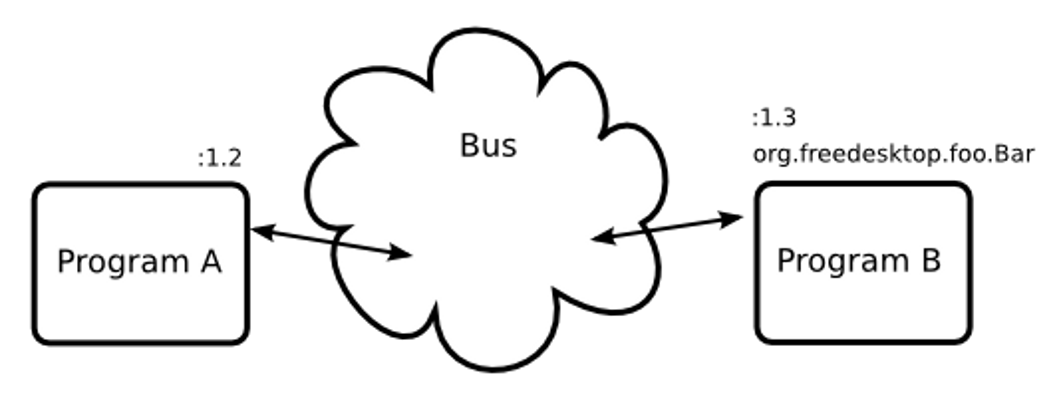
\includegraphics[width=11cm]{fig/dbus-architecture-names.png}
	\caption{D-Bus id and wellknown name example\cite{dbusTP}}
	\label{fig:dbusArchitectureNames}
\end{center}
\end{figure}


The figure \ref{fig:dbusArchitecture} shows an overview of all of the terms described above in a simple diagram.

\begin{figure}[ht]
\begin{center}
	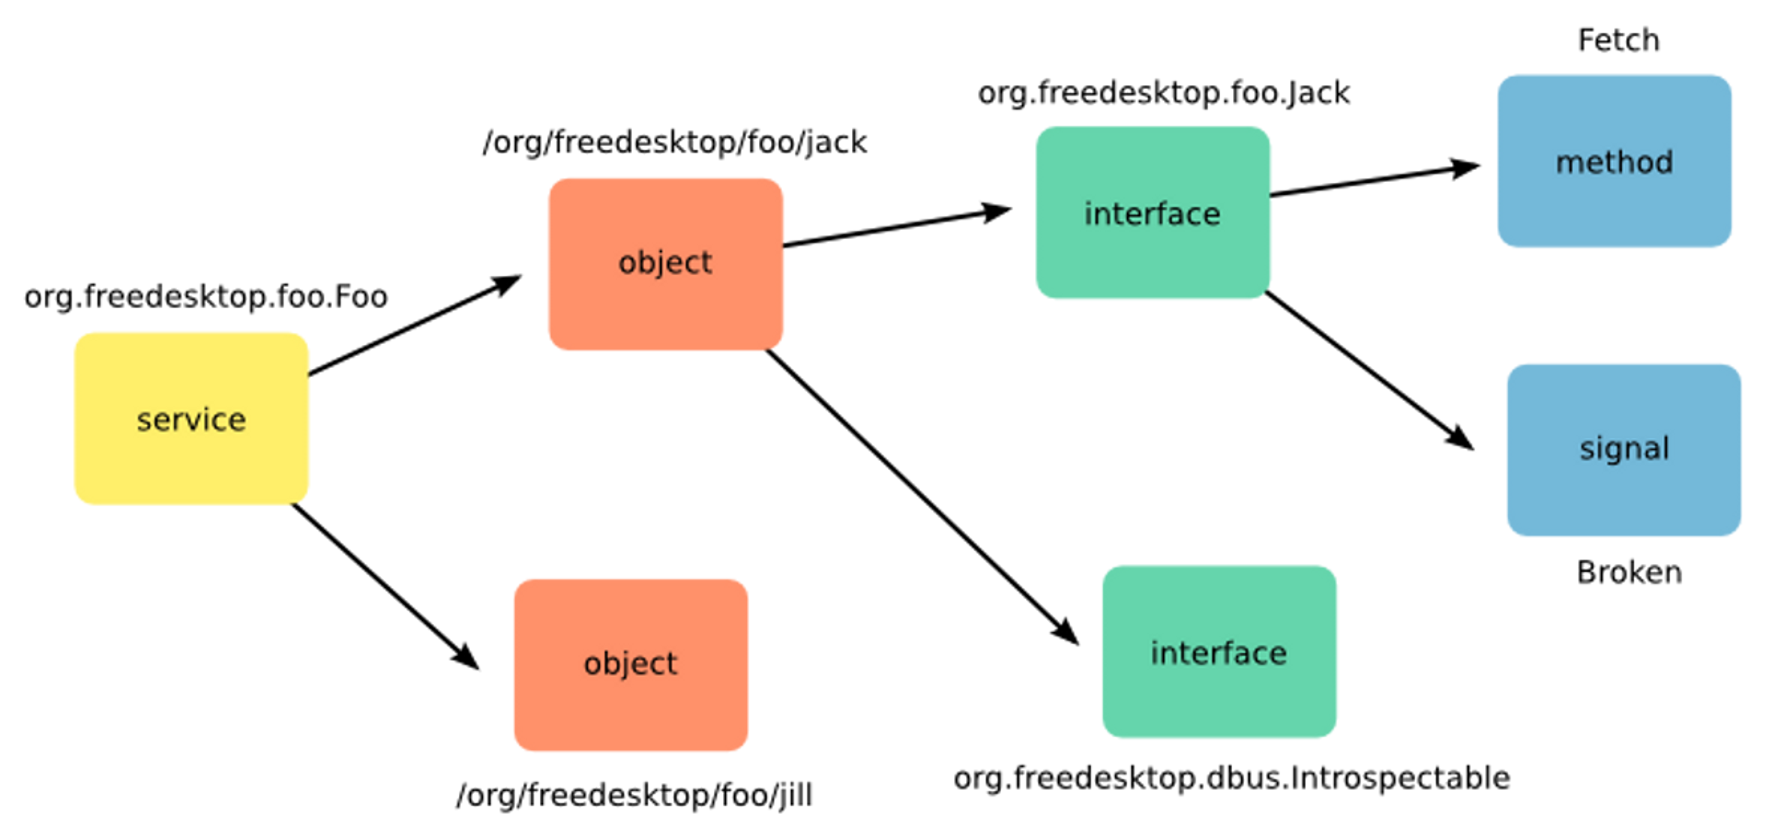
\includegraphics[width=15cm]{fig/dbus-architecture-overview.png}
	\caption{D-Bus architecture\cite{dbusTP}}
	\label{fig:dbusArchitecture}
\end{center}
\end{figure}

D-Bus is a key component of Telepathy framework. Telepathy supports many protocols all of which might provide different capabilites. For example IRC does not support avatars while XMPP does. Eventhough avatar feature is supported by XMPP protocol it might not be supported by the server we are connected to or by the opposite client in case of peer-to-peer connection. The available features are exposed by D-Bus Properties Interface. That is an easy way of determining the protocol, server or client capabilities.\cite{dbus}

\subsection*{Mission Control}
Mission Control is a Telepathy component that implements Account Manager and Channel Dispather and it's primary purpose is to encapsulate those two.\cite{tpWikiMissionControl}\cite{tpWikiBasicTerminology}

\subsection*{Account Manager}
Account Manager is responsible for handling accounts(e.g. XMPP, ICQ, MSN etc.). It is accessible by well-known name on D-Bus - org.freedesktop.Telepathy.AccountManager. A client application first creates an account using the CreateAccount() method, supplying it with ConnectionManager, protocol and display name. Account Manager creates and then as long as the account is active maintains Connection to that account. To create a Connection a Connection Manager is called. An account may be valid or invalid. Valid accounts may establish a Connection, whereas invalid can't. The list of valid and invalid accounts is accessible via ValidAccounts and InvalidAccounts properties respectively.\cite{tpWikiBasicTerminology}\cite{tpWikiAccountManager} 

\subsection*{Account}
When the Account Manager's CreateAccount() is called it returns an Account object. Account object registers with D-Bus and has an object path /org/freedesktop/Telepathy/Account/CM/PROTOCOL/ACCDN. CM stands for Connection Manager(e.g. gabble, salut, butterly etc.), PROTOCOL is substitution for a protocol name and ACCDN is Account Display Name. The Account object implements org.freedesktop.Telepathy.Account interface. Features supported by this interface depend on the protocol used and the server-side software. The Account settings are done via org.freedesktop.Telepathy.Properties interface. All available attributes can be obtained by calling the GetAll() method provided by the Properties Interface. The GetAll() method is very convenient for it returns all the propeties at once in signle D-Bus call. Similarly there is a method for setting all properties at once - Account interface's UpdateParameters() method. The following tables lists all properties of the Account object available. Table \ref{table:configureableProperties} shows properties that can be configured and table \ref{table:nonConfigurableProperties} shows properties just for reading. Some features are available via specified interface, e.g. avatar. Avatar used to be a property, but now it has it's own interface. The Interfaces property of the account lists all interfaces of additional features.\cite{tpWikiBasicTerminology}\cite{tpWikiAccount}

\begin{center}
\begin{table}
	\begin{tabular}{|l|l|p{4.5cm}|p{3cm}|}
		\hline
			\multicolumn{4}{|c|}{{\bf Configurable properties}} \\
		\hline
			{\bf Property} & {\bf Type} & {\bf Description} & {\bf Example} \\
		\hline
			DisplayName & String & Name of the account, used in the account object path. It is usualy displayed by the client application & ``Bob'', ``Work'' \\
		\hline
			Icon & String & Name of an icon to be used for the account. If it is not present the system's icon theme and if not it may be automatically chosen & ``im-jabber'' (jabber's lighbulb), ``im-icq'' (icq's green flower) \\
		\hline
			Enabled & Boolean & Whether or not the Account can go online. Enabled property is different from the valid property of the account with the Account Manager.& True\\
		\hline
		   Nickname & String & This name will appear to other user's that have this account in their contact list, unless they decide to change it on their side of course. & ``Bobman'' \\
		\hline
			AutomaticPresence & SimplePresence* & The status this account will have whenever it is brought online. & \\
		\hline
			RequestedPresence & SimplePresence* & The presence status we wish to change the current status to. & \\
		\hline
			ConnectAutomatically & Boolean & Whether or not a Connection should be requested by the Account Manager automatically. & True \\
		\hline
	\end{tabular}
	\label{table:configureableProperties}
	\caption{Configurable properties of Telepathy Account\cite{tpWikiAccount}}
\end{table}
\end{center}

\begin{center}
\begin{table}
	\begin{tabular}{|l|l|p{8cm}|}
		\hline
			\multicolumn{3}{|c|}{{\bf Nonconfigurable properties}} \\
		\hline
			{\bf Property} & {\bf Type} & {\bf Description} \\
		\hline
			Interfaces & DBus\_Interface[] & A list of interfaces for extra features supported by the account, e.g. org.freedesktop.Telepathy.Account.Interface.Avatar \\
		\hline
			Valid & Boolean & Whether or not this account can be connected(brought online) by the Account Manager. \\
		\hline
		   Connection & Connection & Object path to the connection associated with account if there is any. Otherwise it is set to: '/', e.g. /org/freedesktop/Telepathy/Connection/gabble/jabber/vtheman\_40jabbim\_2ecz0 \\
		\hline
			ConnectionStatus & int & Status of the connection. That is if there is any. \\
		\hline
			ConnectionStatusReason & int & The reason why the last change of status of the connection occured. \\
		\hline
			CurrentPresence & SimplePresence & Current presence of the account. \\
		\hline
	\end{tabular}
	\label{table:nonConfigureableProperties}
	\caption{Configurable properties of Telepathy Account\cite{tpWikiAccount}}
\end{table}
\end{center}


\subsection*{Connection Manager}
Connection Manager supplies Account Manager with Connections. It is not directly used by the client program. Account Manager requests connection for active accounts.

Connection Manager is a protocol-dependent Telepathy component. Different protocols need different Connection Managers. For example if the client application wants to communicate using XMPP/Jabber it has to use Telepathy-gabble and for MSN Telepathy-butterfly is required. Some Connection Managers can communicate via more than one protocol, for example Telepathy-haze. To see what protocols are supported there is ListProtocols() method implemented by the Connection Manager.\cite{tpWikiBasicTerminology}\cite{tpWikiConnectionManager}

\subsection*{Connection}
Connection represents an active protocol session. It is associated with an Account and is created by Connection Manager based on a request of the Account Manager. Connection implements org.freedesktop.Telepathy.Connection interface and additional interfaces depending on the protocol. List additional interfaces available can be retrieved by checking the Interfaces property. The most common interfaces are listed below\cite{tpWikiConnection}:

\begin{itemize}

	\item {\bf Contacts} - used to get as much information about a contact as asked in one D-Bus call.

	\item {\bf Aliasing} - serves for setting aliases for contacts and checking if the contacts have changed their alias themselves. 

	\item {\bf Avatars} - interface to one of the most popular protocol features. Allows users to set their avatars and retrieve other users' avatars.

	\item {\bf ContactCapabilities} - retrieves capabilities of contacts' Clients to see what features they support. Checks for example for VoIP or file transfer support.

	\item {\bf Location} - lets user publish his or her current location as well as find out his or her contacts' whereabouts. 

\end{itemize}


\subsection*{Channel Dispatcher}
This component handles Channels incoming from active Connections of valid Accounts. Channel Dispatcher monitors available or activatable Telepathy Clients through D-Bus. Clients register with user's session D-Bus and provide a CLIENT\_NAME.client file. Both of those serve as a way to publish Client's properties including a channel filter. The Channel Dispatcher based on these properties knows what kind of a client it is and what type of channels it is interested in (channel filter). If the Client is running then the properties are acquired via the Client interface. If the client is not running and is activatable then the .client file is used by Channel Dispatcher to pre-look up the properties and if they match the incoming Channel, the Client is activate.So providing the .client file only makes sense for activatable Clients.  

When a Channel comes in from one of the Connections Channel Dispatcher notifies appropriate Clients. There are three kinds of clients - Observer, Approver and Handler(see \ref{subsect:tpClient}). The Channel is dispatched to all Observers and all Approvers with a matching channel filter. The Approvers choose Handler to handle the Channel. Should the Client fail, Channel Dispatcher may recover from such error and look for another Handler.\cite{tpWikiBasicTerminology}\cite{tpWikiChannelDispatcher}  


\subsection*{Channel}
Channel allows the local client to exchange various kind of data with a remote server. It is associated with a Connection and always implements at least two interfaces. The first is org.freedesktop.Telepathy.Channel and the second depends on the Channel type. Channels for text messaging will be of type Text and will implement org.freedesktop.Telepathy.ChannelType.Text interface. The following list shows most common types of Channels\cite{tpWikiChannel}:

\begin{itemize}

	\item {\bf ContactList} - used to get information of contacts in user's contact list.

	\item {\bf Text} - designed for exhanging text messages. 

	\item {\bf Call} - used for VoIP and video calls. 

	\item {\bf FileTransfer} - Channel for sending and receiving files.

	\item {\bf ContactSearch} - is used when a user wants to find a contact on a server.

\end{itemize}

Channels are created using two methods - CreateChannel() and EnsureChannel(). These methods are implemented by both Channel Dispatcher and Connection. When calling either of those methods on Channel Dispatcher the resulting Channel will go through the procedure of looking for handler as described above. When using directly the connection the calling application must handle the Channel itself as the Channel Dispatcher will not interfere. It is also possible to supply the Channel Dispatcher with a preferred handler and thus achieve the same effect. It is better to use the Channel Dispatcher for if the client should fail it may dispatch the Channel to another handler.\cite{tpWikiRequestingChannels}\cite{incomingChannels}

Both CreateChannel() and EnsureChannel() methods provide a Channel. The difference between the two is that CreateChannel() creates actual new Channel whereas EnsureChannel() will attemp to reuse an existing Channel with the same properties. If there is no Channel to be reused or it is being used by a different application than it creates a new Channel, just like CreateChannel(). Typicaly CreateChannel() is used for FileTransfer and ContactSearch and EnsureChannel() for Text, StreamedMedia and ContactLists Channels.\cite{tpWikiRequestingChannels} 

\subsection*{Client}\label{subsect:tpClient}
Client is an application that wants to use Telepathy. It needs to register a well-known name in org.freedesktop.Telepathy.Client namespace, e.g. Empathy registers org.freedesktop.Telepathy.Client.Empathy. Then it provides a .client file where purpose of which is described above. Telepathy defines three types of clients - Observer, Approver and Handler. All of these need to provide appropriate channel filter, e.g. Oberver provides ObserverChannelFilter. Based on the published filter the Channel Dispatcher dispatches an incoming Channel to the Client or not.\cite{tpWikiClient}  

Observers are called upon a creation of a new Channel. They monitor Channels and provide the acquired information to user. The observers have different functions based on the type of observed Channel, e.g. Text Channel observer might serve as a logger and FileTransfer observer as a file transfer progress monitor. Observer is must not interfere except for when the user interaction like hitting the cancel button in a file transfer progress window.\cite{tpWikiClient}     

Approver is a Telepathy Client that is supposed to accept the incoming Channel and decide, which Handler it is dispatched to. The Channel Dispatcher provides Approvers with a list of possible Handlers. Approver notifies the user of a new Channel and lets him or her decide whether to accept or reject it. Similarly the user is allowed to choose which Handler will handle the Channel. Handler might also be chosen by the Approver itself. Approver does not call methods just like the Observer. Calling methods is up to the Handlers. For example if there is an incoming file transfer the Approves lets user decide whether to accept it or not, but the AcceptFile method will be called by the chosen Handler.\cite{tpWikiClient}  

The last client is Handler. Handler does all the interaction with the Channel. A typical example of a Handler is chat-window. It displays messages and allows the user to send text messages back.\cite{tpWikiClient}  

\subsection*{Handle}
Telepathy handles represent objects like contact, roster, chatroom etc. It is a number, assigned by Connection the object is related to, that identifies the object. In addition to the numeric id handles also have a string id(e.g. chatroom could have a string id makneto@jabber-discussion.com). Depending on the protocol resource the handle represents it is of an apropriate type(Handle\_type property). Handles with different types may have the same numeric id. When comparing handles it should be always done by comparing the numeric id's, assuming we are comparing handles of the same type.\cite{tpWikiHandle} 


\begin{figure}[ht]
\begin{center}
	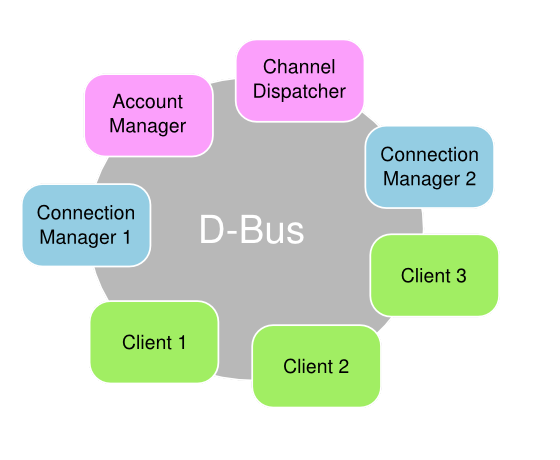
\includegraphics[width=10cm]{fig/telepathy-components-dbus.png}
	\caption{Telepathy components registered with user session D-Bus.\cite{tpWikiClient}}
	\label{fig:telepathyComponentsDbus}
\end{center}
\end{figure}

The figure \ref{fig:telepathyComponentsDbus}

%\section{Telepathy language bindings}
%Telepathy clients may be written using language bindings. These bindings must provide D-Bus API. 
%Telepathy-glib, Telepathy-python
%Telepathy-qt4

\section{Empathy}
Empathy is a multiprotocol instant messaging application based on Telepathy. In the terms described above Empathy is a Telepathy client. It is written in python using Telepathy-python bindings. Empathy registers a well-known name with D-Bus and communicates with Telepathy components to provide the communication services. Empathy supports text messaging, file transfer, voice and video calls over various protocols. Supported protocol include Google Talk, XMPP/Jabber, MSN, IRC, AIM Facebook, Yahoo!, Gau Gadu, and ICQ. For some of those protocols like Google Talk and XMPP voice and video calls implemented. The suppport of the protocols depend on Telepathy Connection managers installed. Additional functionality includes sharing users' whereabouts among themselves, automatic reconnection when internet connection is reestablished and automatic changes of presence to away and extended away.\cite{empathyGnome}

The current stable version of Empathy is 2.32.2 and it is a default communication application in GNOME releases since version 2.24 instead of Pidgin. It's GUI is takes after Gossip, which is an older IM application for GNOME. 

% =========================================================================================================================
% =========================================================================================================================

\chapter{Audio and video streaming protocols}

% =========================================================================================================================
% =========================================================================================================================

%\chapter{Implementation}

% =========================================================================================================================
% =========================================================================================================================

\chapter{Conclusion}
Závěrečná kapitola obsahuje zhodnocení dosažených výsledků se zvlášť vyznačeným vlastním přínosem studenta. Povinně se zde objeví i zhodnocení z pohledu dalšího vývoje projektu, student uvede náměty vycházející ze zkušeností s řešeným projektem a uvede rovněž návaznosti na právě dokončené projekty.

